\documentclass[12pt]{article}

\usepackage[utf8]{inputenc}
\usepackage[margin=1in]{geometry}
\renewcommand{\baselinestretch}{1}
\usepackage{indentfirst}

\usepackage{amsmath, amssymb}

\usepackage{hyperref}
\usepackage{cleveref}
\usepackage{graphicx}
\usepackage{float}
\graphicspath{{./figs/}}

\begin{document}

\begin{center}\begin{LARGE}
\textbf{Assignment 5: Results/Description}
\end{LARGE}\end{center}

\section*{Problem 1}

For this problem I have written two programs (\texttt{myFTCS} and
\texttt{myCN}) to solve the following problem. These may be compiled all
together with a \texttt{make all} as shown below.

\begin{figure}[H]
    \centering
    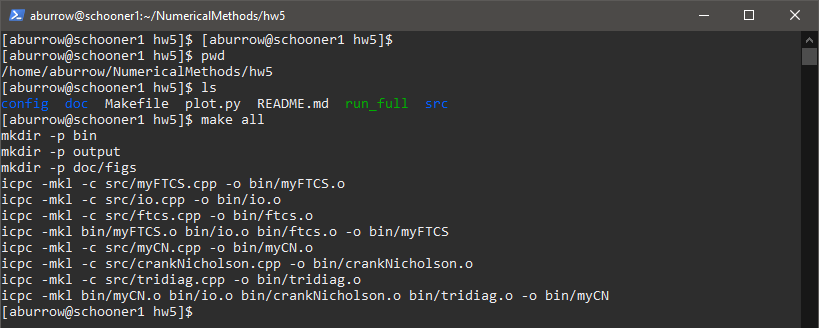
\includegraphics[width=1\textwidth]{compile}
    \label{fig:compile}
\end{figure}

This generates executables \texttt{myFTCS} and \texttt{myCN} in the ``./bin''
directory, which may be run one at a time. There is also a \texttt{plot.py} in
the root which may be run to generate plots from the output of the executables.
However, to run all these programs at once, I have also included a
\texttt{run\_full} bash script that may be executed for convenience.

In this problem, I use (a) the FTCS method and (b) the Crank-Nicolson method
to solve the diffusion equation
$$
\begin{aligned}
\frac{\partial n}{\partial t}
&= \frac{\partial^2 n}{\partial x^2}.
\end{aligned}
$$

\subsection*{(a)}

Below I run the program that demonstrates solving our differential equation
using the FTCS method:
\begin{figure}[H]
    \centering
    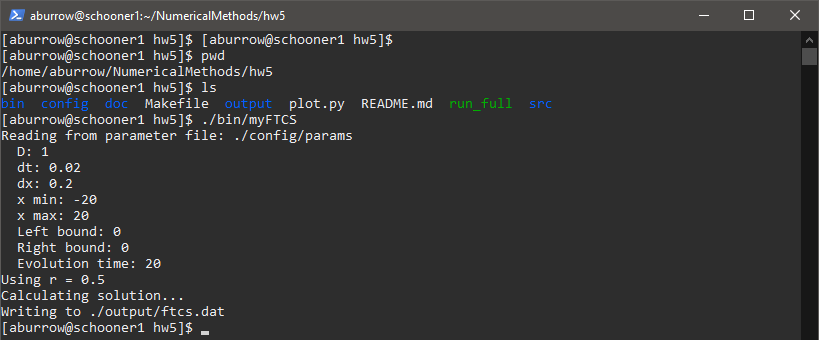
\includegraphics[width=1\textwidth]{myFTCS}
    \label{fig:myFTCS}
\end{figure}

This was equation was solved over $t \in [0, 20]$ with the boundary conditions
given in the problem. First, I solved this using $\Delta t = 0.2$ ($r = 0.5$),
and the result is shown in \autoref{fig:ftcs-r0.500}. We see clear diffusion in
this solution, so the solver works as intended.

\begin{figure}[ht]
    \centering
    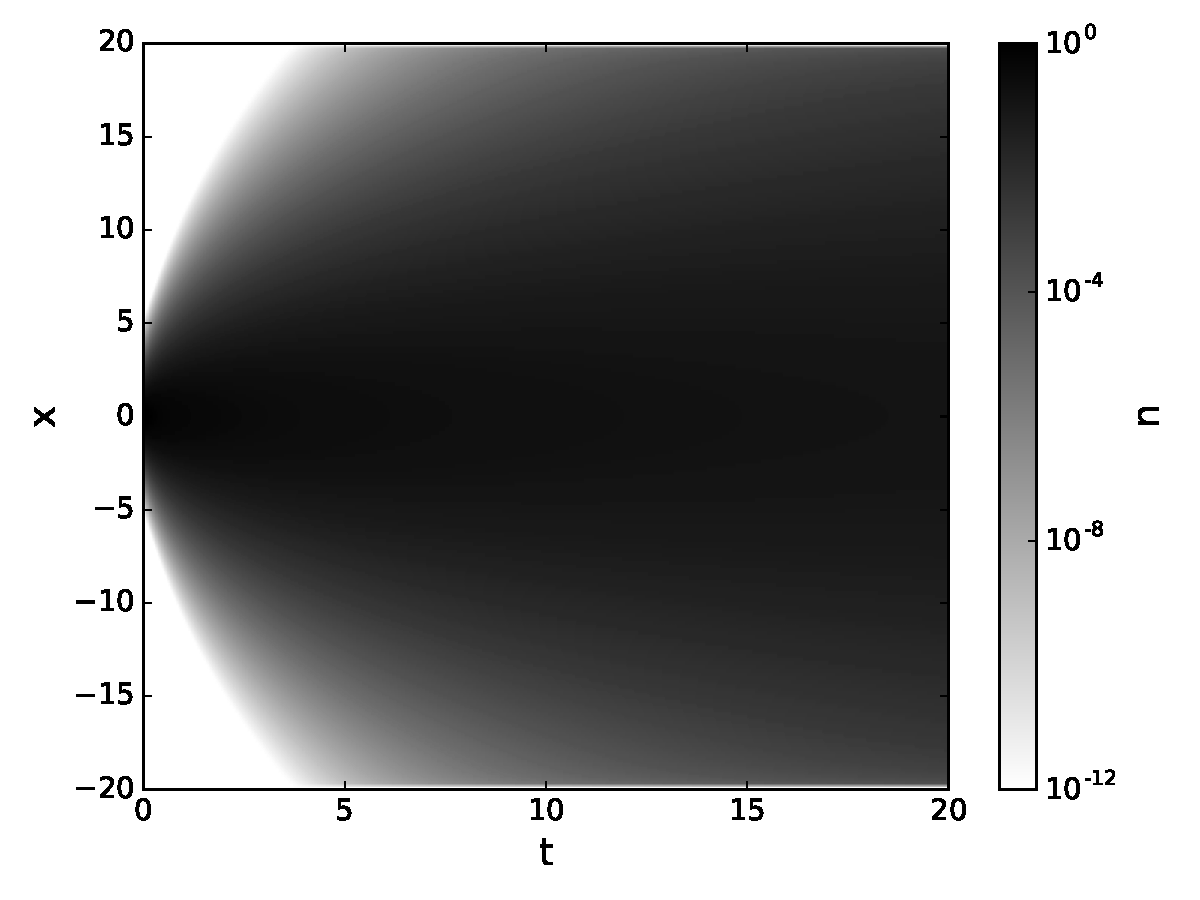
\includegraphics[width=0.8\textwidth]{ftcs-r0.500}
    \caption{Solution using the FTCS method with $r = 0.5$.}
    \label{fig:ftcs-r0.500}
\end{figure}

Next, I change my time step to be $\Delta t = 0.266$ ($r = 0.665 > 0.5$), and
the result is given in \autoref{fig:ftcs-r0.665}. We see clearly that a
divergence has occured as expected, due to the stability condition of the FTCS
method. The solution apparently becomes completely unstable at about t = 2.5.

\begin{figure}[ht]
    \centering
    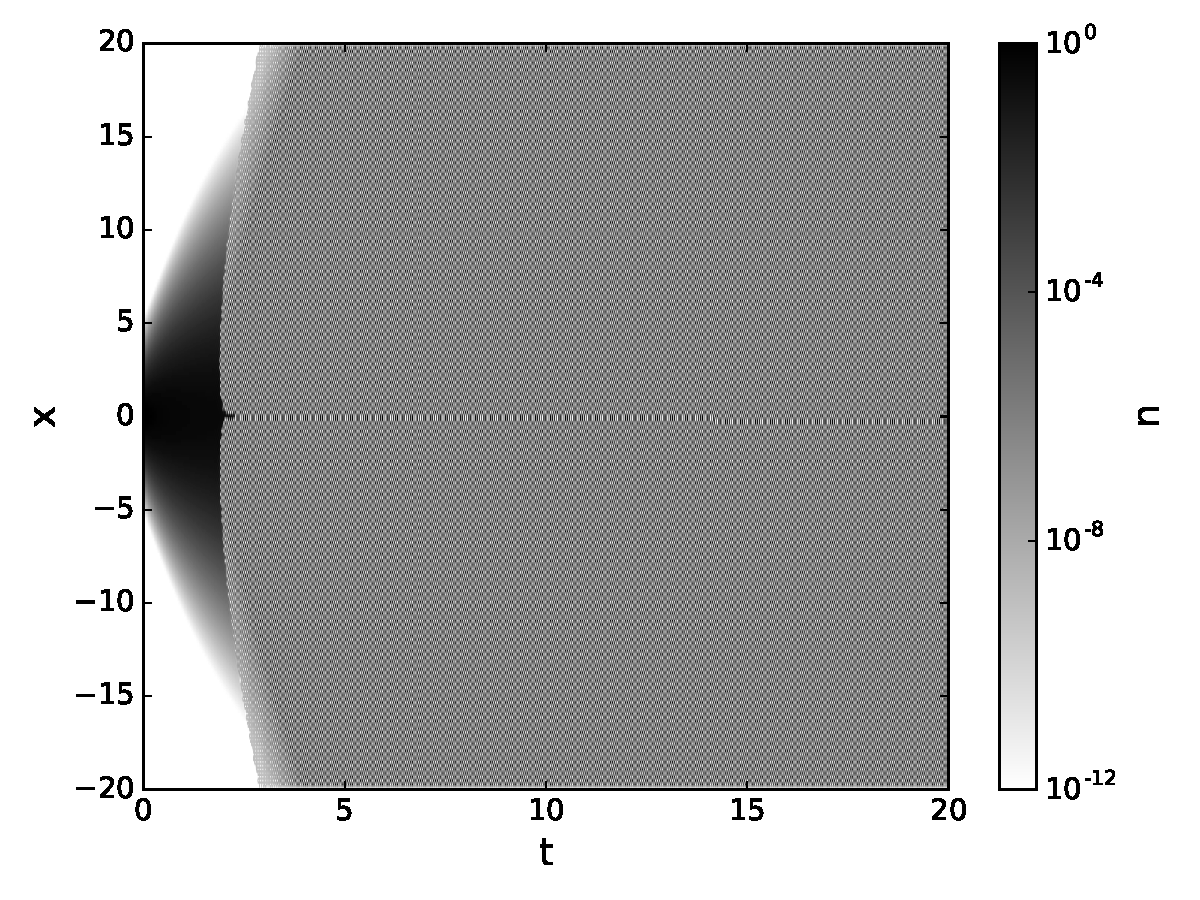
\includegraphics[width=0.8\textwidth]{ftcs-r0.665}
    \caption{Solution using the FTCS method with $r > 0.5$.}
    \label{fig:ftcs-r0.665}
\end{figure}

\subsection*{(b)}

Below I run the program that demonstrates solving our differential equation
using the Crank-Nicolson method:
\begin{figure}[H]
    \centering
    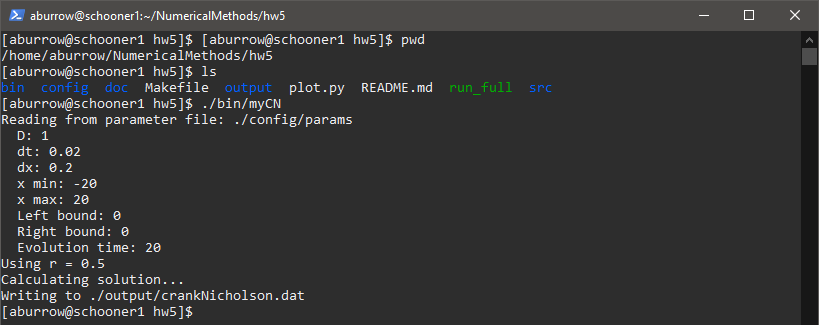
\includegraphics[width=1\textwidth]{myCN}
    \label{fig:myCN}
\end{figure}

For this method I use the same boundary conditions as before over the same time
period. Again I calculate the solution with $\Delta t = 0.2$, and the result
(shown in \autoref{fig:crankNicolson-r0.500}) is the same as that in
\autoref{fig:ftcs-r0.500}.

\begin{figure}[ht]
    \centering
    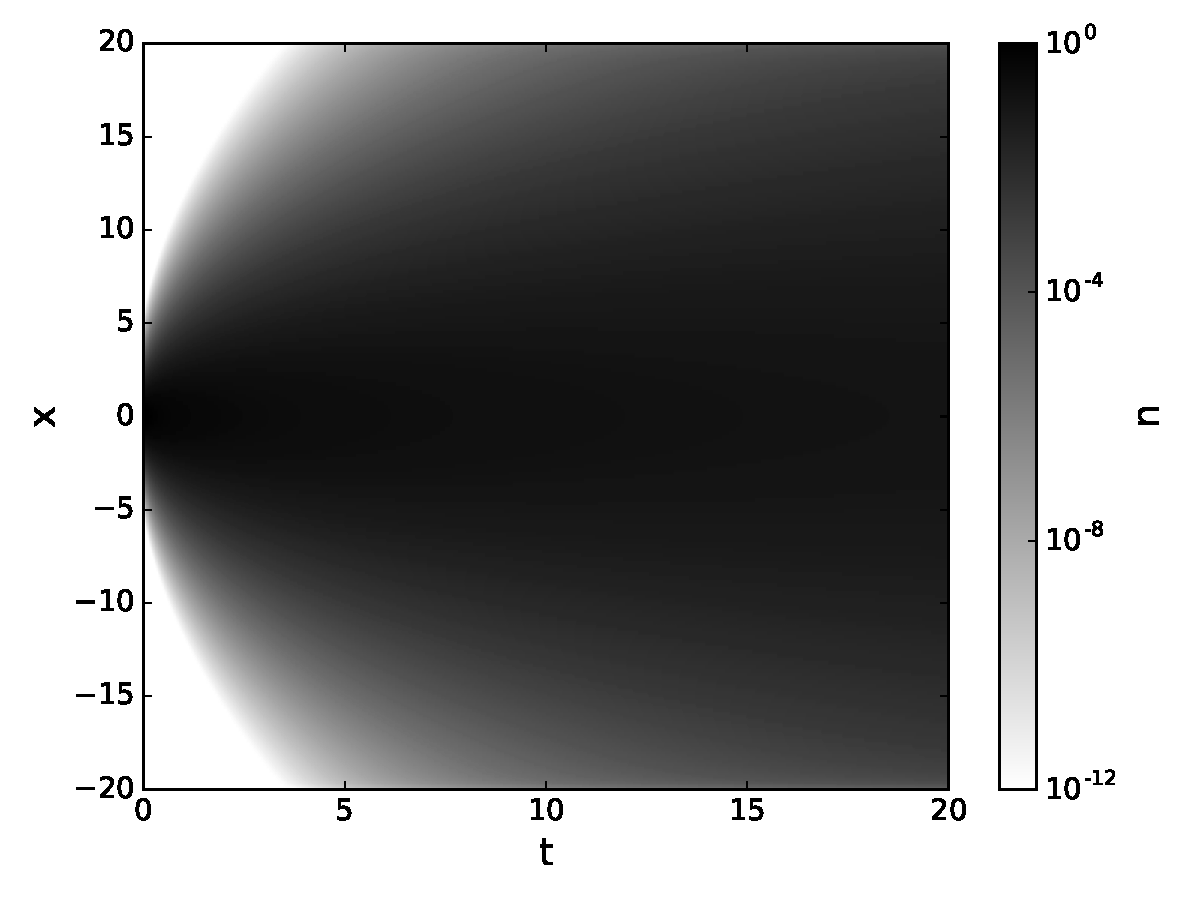
\includegraphics[width=0.8\textwidth]{crankNicolson-r0.500}
    \caption{Solution using the Crank-Nicolson method with $r = 0.5$.}
    \label{fig:crankNicolson-r0.500}
\end{figure}

However, when I use $\Delta t = 0.266$ to calculate the solution (shown in
\autoref{fig:crankNicolson-r0.665}), we do not see any unstability, unlike
for the FTCS case. Instead, we find the intended solution. I was not able to
find any reasonable value of $\Delta t$ that led to an unstable solution with
the Crank-Nicolson method. In general, this should not happen, as it is proven
to have no Courant condition for stability (however you still need it for
accuracy).

\begin{figure}[ht]
    \centering
    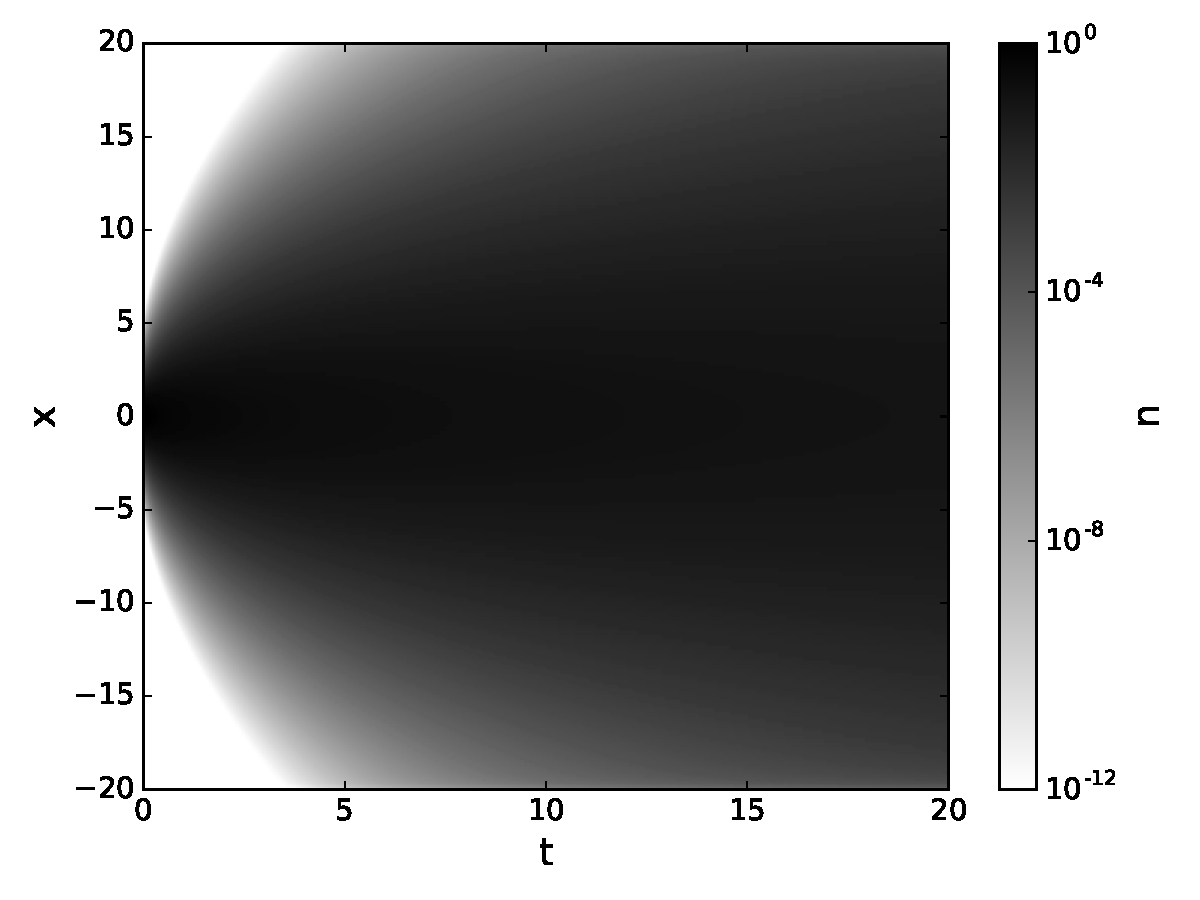
\includegraphics[width=0.8\textwidth]{crankNicolson-r0.665}
    \caption{Solution using the Crank-Nicolson method with $r > 0.5$.}
    \label{fig:crankNicolson-r0.665}
\end{figure}


\end{document}
